%%%%%%%%%%%%%%%%%%%%%%%%%%%%%%%%%%%%%%%%%%%%%%%%%%%%%%%%%%%%%%%%%
\chapter{INTRODUCTION TO MACHINE LEARNING}
\label{ch:CH4}
%%%%%%%%%%%%%%%%%%%%%%%%%%%%%%%%%%%%%%%%%%%%%%%%%%%%%%%%%%%%%%%%%

In this chapter, we start with the basics of machine learning. Then we mention cross-validation approach, which is a model evaluation technique, and the regularization concept. Finally, we end the section with the ML algorithms used in the thesis. The Figure~\ref{basic_ml} shows a simple road-map of a machine learning task.

\begin{figure}[h]
	\centering
	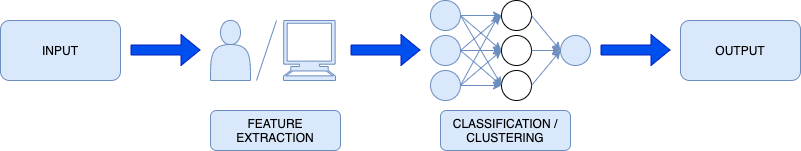
\includegraphics[width=\linewidth]{fig/basic_ml.png}
	\vspace*{2mm}
	\caption{Sample machine learning road map.}
	\label{basic_ml}
\end{figure}

\section{The Basics of Machine Learning}

The goal of machine learning (ML) is to learn from available data or experiences to solve a given problem. A traditional ML pipeline may be listed as follows:

\begin{itemize}
    \item defining the problem to solve,
    \item collecting the data for training and testing,
    \item designing or extracting the features describing data,
    \item training the model to optimize the loss function by tuning the parameters through experiments, and
    \item testing the model to evaluate the performance of trained model on unseen test data.
\end{itemize}

The majority of the problems in ML classified as either supervised or unsupervised learning approaches. \textcolor{purple}{Clustering as an example for unsupervised learning, and classification and regression as two examples for supervised learning are given in Figure~\ref{clustering_classification_regression}.}

\begin{figure}[h]
	\centering
	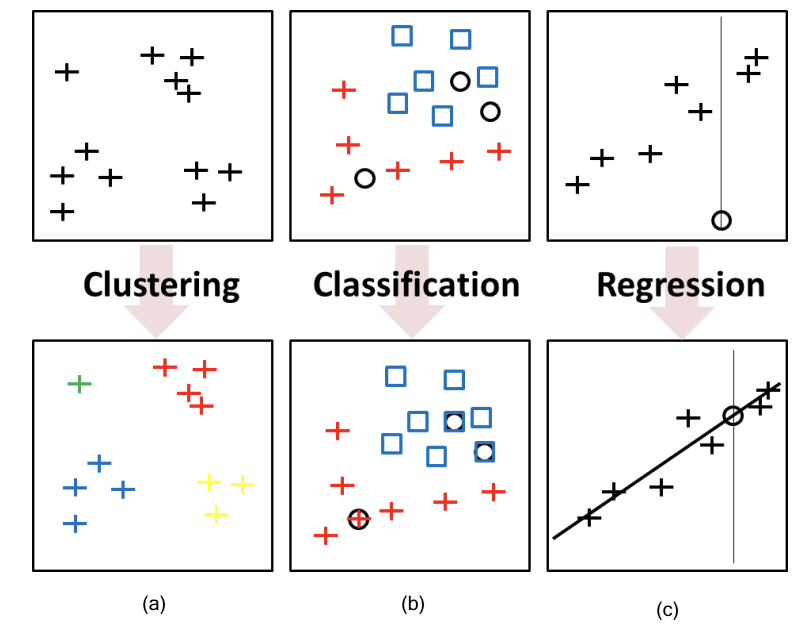
\includegraphics[width=.8\linewidth]{fig/clustering_classification_regression.png}
	\caption{(a) Clustering problem, (b) Classification problem, and (c) Regression problem \cite{parallel_linear_algebra}.}
	\label{clustering_classification_regression}
\end{figure}

\subsection{Supervised Learning}

Supervised learning is a ML method that establishes a relationship between each attribute of data feature map and its target value. Estimating the output value for each new datum is the main goal. All true target values are known during training and testing. These known true values are used to construct the trained model and to evaluate the testing performance. Regression and classification problems are solved by supervised learning approaches.

The task in this thesis includes a data set where each datum has its true label value. Thus, all ML models used in this thesis are supervised learning algorithms.

\subsection{Unsupervised Learning}

The problems having data with unknown true values are solved by unsupervised learning. \textcolor{purple}{Some data sets can be deliberately left unlabeled since it is too hard to label the data and requires too much time, expert people, or special devices to label. On the other hand, not all problems needs to be classified, there are problems that only needs to be grouped. Clustering tasks are constructed on these kind of data sets and solved by unsupervised learning.}

\section{Cross-Validation}

As in deep learning, over-fitting and under-fitting creates serious problems in machine leaning. Cross-validation (CV) methods can be used to overcome these problems. In the CV method, all the data is divided into train and test sets. Here, it should be noted that the train and test data sets must be strictly separated from each other, and any sample on test set should not be seen during training process.

\subsection{K-Fold Cross-Validation}

In K-Fold CV, K is the hyper-parameter to tune that defines the number of folds during partitioning. The choice of K must be greater than 1 and less than the number of data points. All data is divided into K folds of the same (if possible) or different sizes. The folds are enumerated from 1 to K. Here, the model is evaluated and tested $(K-1)$ times. On each iteration $i$, where $i$ is an integer from 1 to K, the $i^{th}$ fold is chosen as the test set and the rest as the train set, and model forgets what it learned previously and starts from zero. Otherwise, the test data on the $(i+1)^{th}$ iteration takes place in the train set on the $i^{th}$ iteration and is learned by the model. A sample illustration of K-Fold cross-validation process can be seen in the Figure~\ref{k_fold_cv}.

\begin{figure}[h]
	\centering
	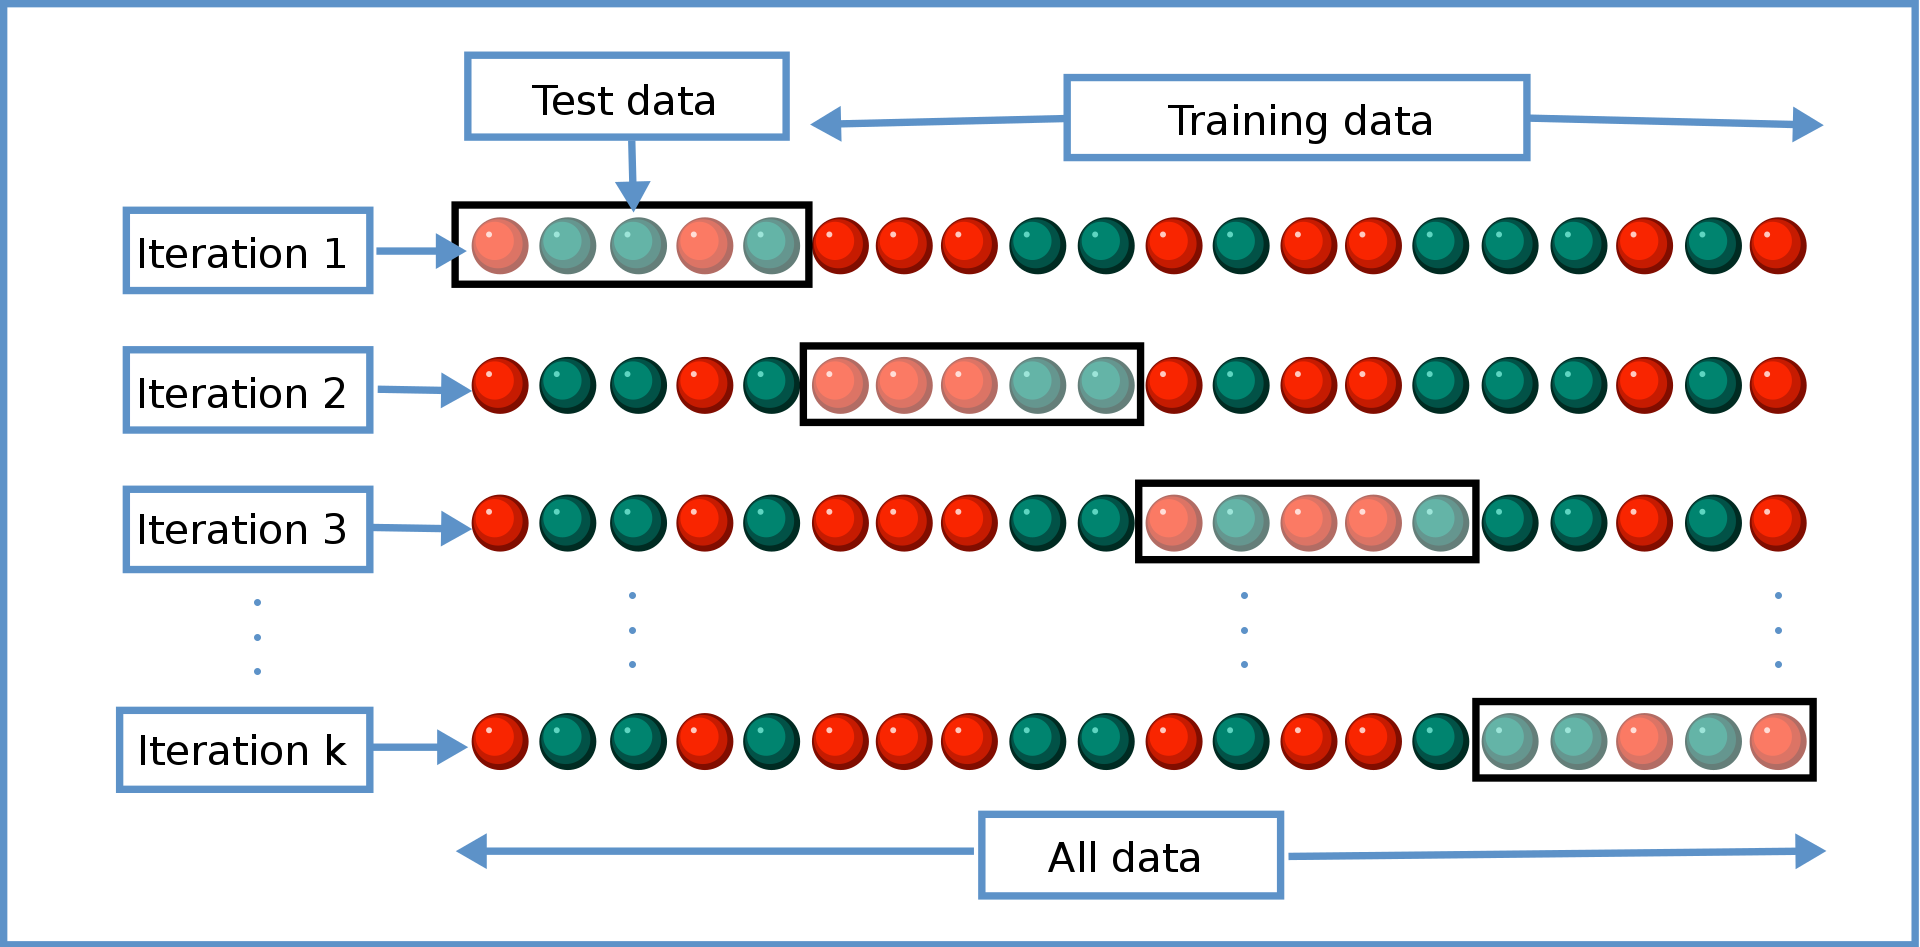
\includegraphics[width=.8\linewidth]{fig/k_fold_cv.png}
	\vspace*{2mm}
	\captionfootnotemark{K-fold cross-validation.}
	\label{k_fold_cv}
\end{figure}
\footnotetext{Retrieved from: \hyperrefurl{https://towardsdatascience.com/cross-validation-c4fae714f1c5} on April 10, 2021.}


\subsection{Leave-One-Out}

If the K of K-Fold CV is chosen as the number of data, say N, it is a special case of CV and called as leave-one-out (LOO) method. As a convenience, all data are enumerated from 1 to N. Thus, model is evaluated and tested for N times. On each iteration $i$, where $i$ is an integer from 1 to N, the $i^{th}$ datum is chosen as the test sample and rest as the train set, and model forgets what it learned previously and starts from zero. Otherwise, the test sample on the current iteration takes place in the train set on the previous iteration and is learned by the model.

Briefly, LOO is the K-Fold CV where the number of folds is chosen as the number of data.

\section{Regularization}
\label{sec:CH5_regularization}

As discussed in Section~\ref{sec:CH3_the_basics_of_optimization}, the training process includes the optimization of corresponding loss function in machine learning. To minimize the loss and obtain the more optimized results, the regularization term is applied to the objective loss function. In general, the regularized loss function for supervised learning can be motivated as:

\be
\label{eq:general_regularized_loss}
\sum_{(x^{i}, y^{i} \in D)} \Big(\frac{Error(f_{w}(x^i), y^{i})}{n}\Big) + \lambda R(f_{w}), 
\ee

where $n$ is the number of training samples, $D$ is the training feature set with $x^{i}$ as training input and $y^{i}$ as the corresponding target output, $f_{w}$ is the mapping function between feature map and target values, $\lambda$ is a real number hyper-parameter greater than or equal to zero controlling the effect of regularization term, and $R$ is the regularization term. 

Notice that, if $\lambda$ is chosen as too high, the regularizer drowns out the loss function; and, if $\lambda$ is chosen as zero, there is no regularization. $\lambda$ is usually chosen between $0$ and $0.1$; however, it must be tuned for the corresponding task.

In addition, the regularization term $R$ has a constraint such that $R(f_{w}) \leq \textbf{$\mu$}$ for an appropriate real valued constant $\textbf{$\mu$}$. This constraint enables to control the magnitude of regularization, and fine tune the hyper-parameter of regularizer.

The regularization is also called as penalty to the objective function. In this section, we focus on LASSO penalty and Ridge regression concepts which are used in this thesis.

\subsection{L1 Regularization}

L1 regularization term, which is known as LASSO, only penalizes the coefficients large in magnitude. The LASSO penalty is in the form of:

\be
\label{eq:lasso_term}
\lambda \norm{\mathbf{w}}_{1},
\ee

where $\textbf{w}$ is the the weight coefficients to estimate and $\norm{.}_{1}$ is the L1 norm such that:

\be
\label{eq:l1_norm}
\norm{\mathbf{w}} = \sum_{i=1}^{p} | w_{i} |,
\ee

for a vector $\textbf{w}$ with length of $p$. LASSO penalty may produce non-unique solutions \cite{lasso_penalty}.

\subsection{L2 Regularization}

L2 regularization term is known as ridge regression. The penalty term in ridge regression is in the form of:

\be
\label{eq:ridge_term}
\lambda \norm{\mathbf{w}}_{2}^{2},
\ee

where $\textbf{w}$ is the weight coefficients to estimate, and $\norm{.}_{2}^{2}$ is the squared L2 norm such that:

\be
\label{eq:l2_norm}
\norm{\textbf{w}}_{2}^{2} = \sum_{i=1}^{p} w_{i}^2,
\ee

for a vector $\textbf{w}$ with length of $p$. 

Since L1 regularizer takes the absolute value and L2 regularizer takes the square, the cost of outlier samples exponentially increase. For this reason, L2 regularization is less robust to outliers than L1 regularizer.

\section{Machine Learning Algorithms}

In this section, the state-of-the-art ML algorithms used in the thesis are introduced and detailed. 
\subsection{Support Vector Machines}

The current support-vector machines algorithm is proposed by Corinna Cortes and Vladimir Vapnik at 1995 \cite{svm_original}. While it is mainly used for supervised learning problems, the version for clustering, which is stated as support-vector clustering \cite{support_vector_clustering}, can be used for unsupervised learning problems.

A support vector machine (SVM) constructs a set of hyper-planes in a high-dimensional or an infinite-dimensional space. It is usually desired to have samples far away from hyper-planes to achieve a good separation result. The parallel hyper-plane to a SVM hyper-plane including the nearest samples of a class, which are the support-vectors, is called as the margin of that class to the corresponding hyper-plane, and larger margins provides lower generalization errors for the classifier. 

In this thesis, we have a binary classification problem; thus, our space is two-dimensional and we have one hyper-plane that has two margins in total. The hyper-planes and, in turn, margins differ depending on the kernel function used. The original hyper-plane algorithm proposed by Vapnik \cite{svm_original} is the linear classifier whose kernel function is clearly called as linear kernel. However, to create nonlinear hyper-planes, Bernhard Boser, Isabelle Guyon  and Vladimir Vapnik \cite{svm_kernel} suggest replacing the linear function with another nonlinear kernel functions. This technique is called as kernel trick. An illustration about how SVM creates the hyper-planes can be viewed in the Figure~\ref{fig:simple_svm}.

\begin{figure}[h]
	\centering
	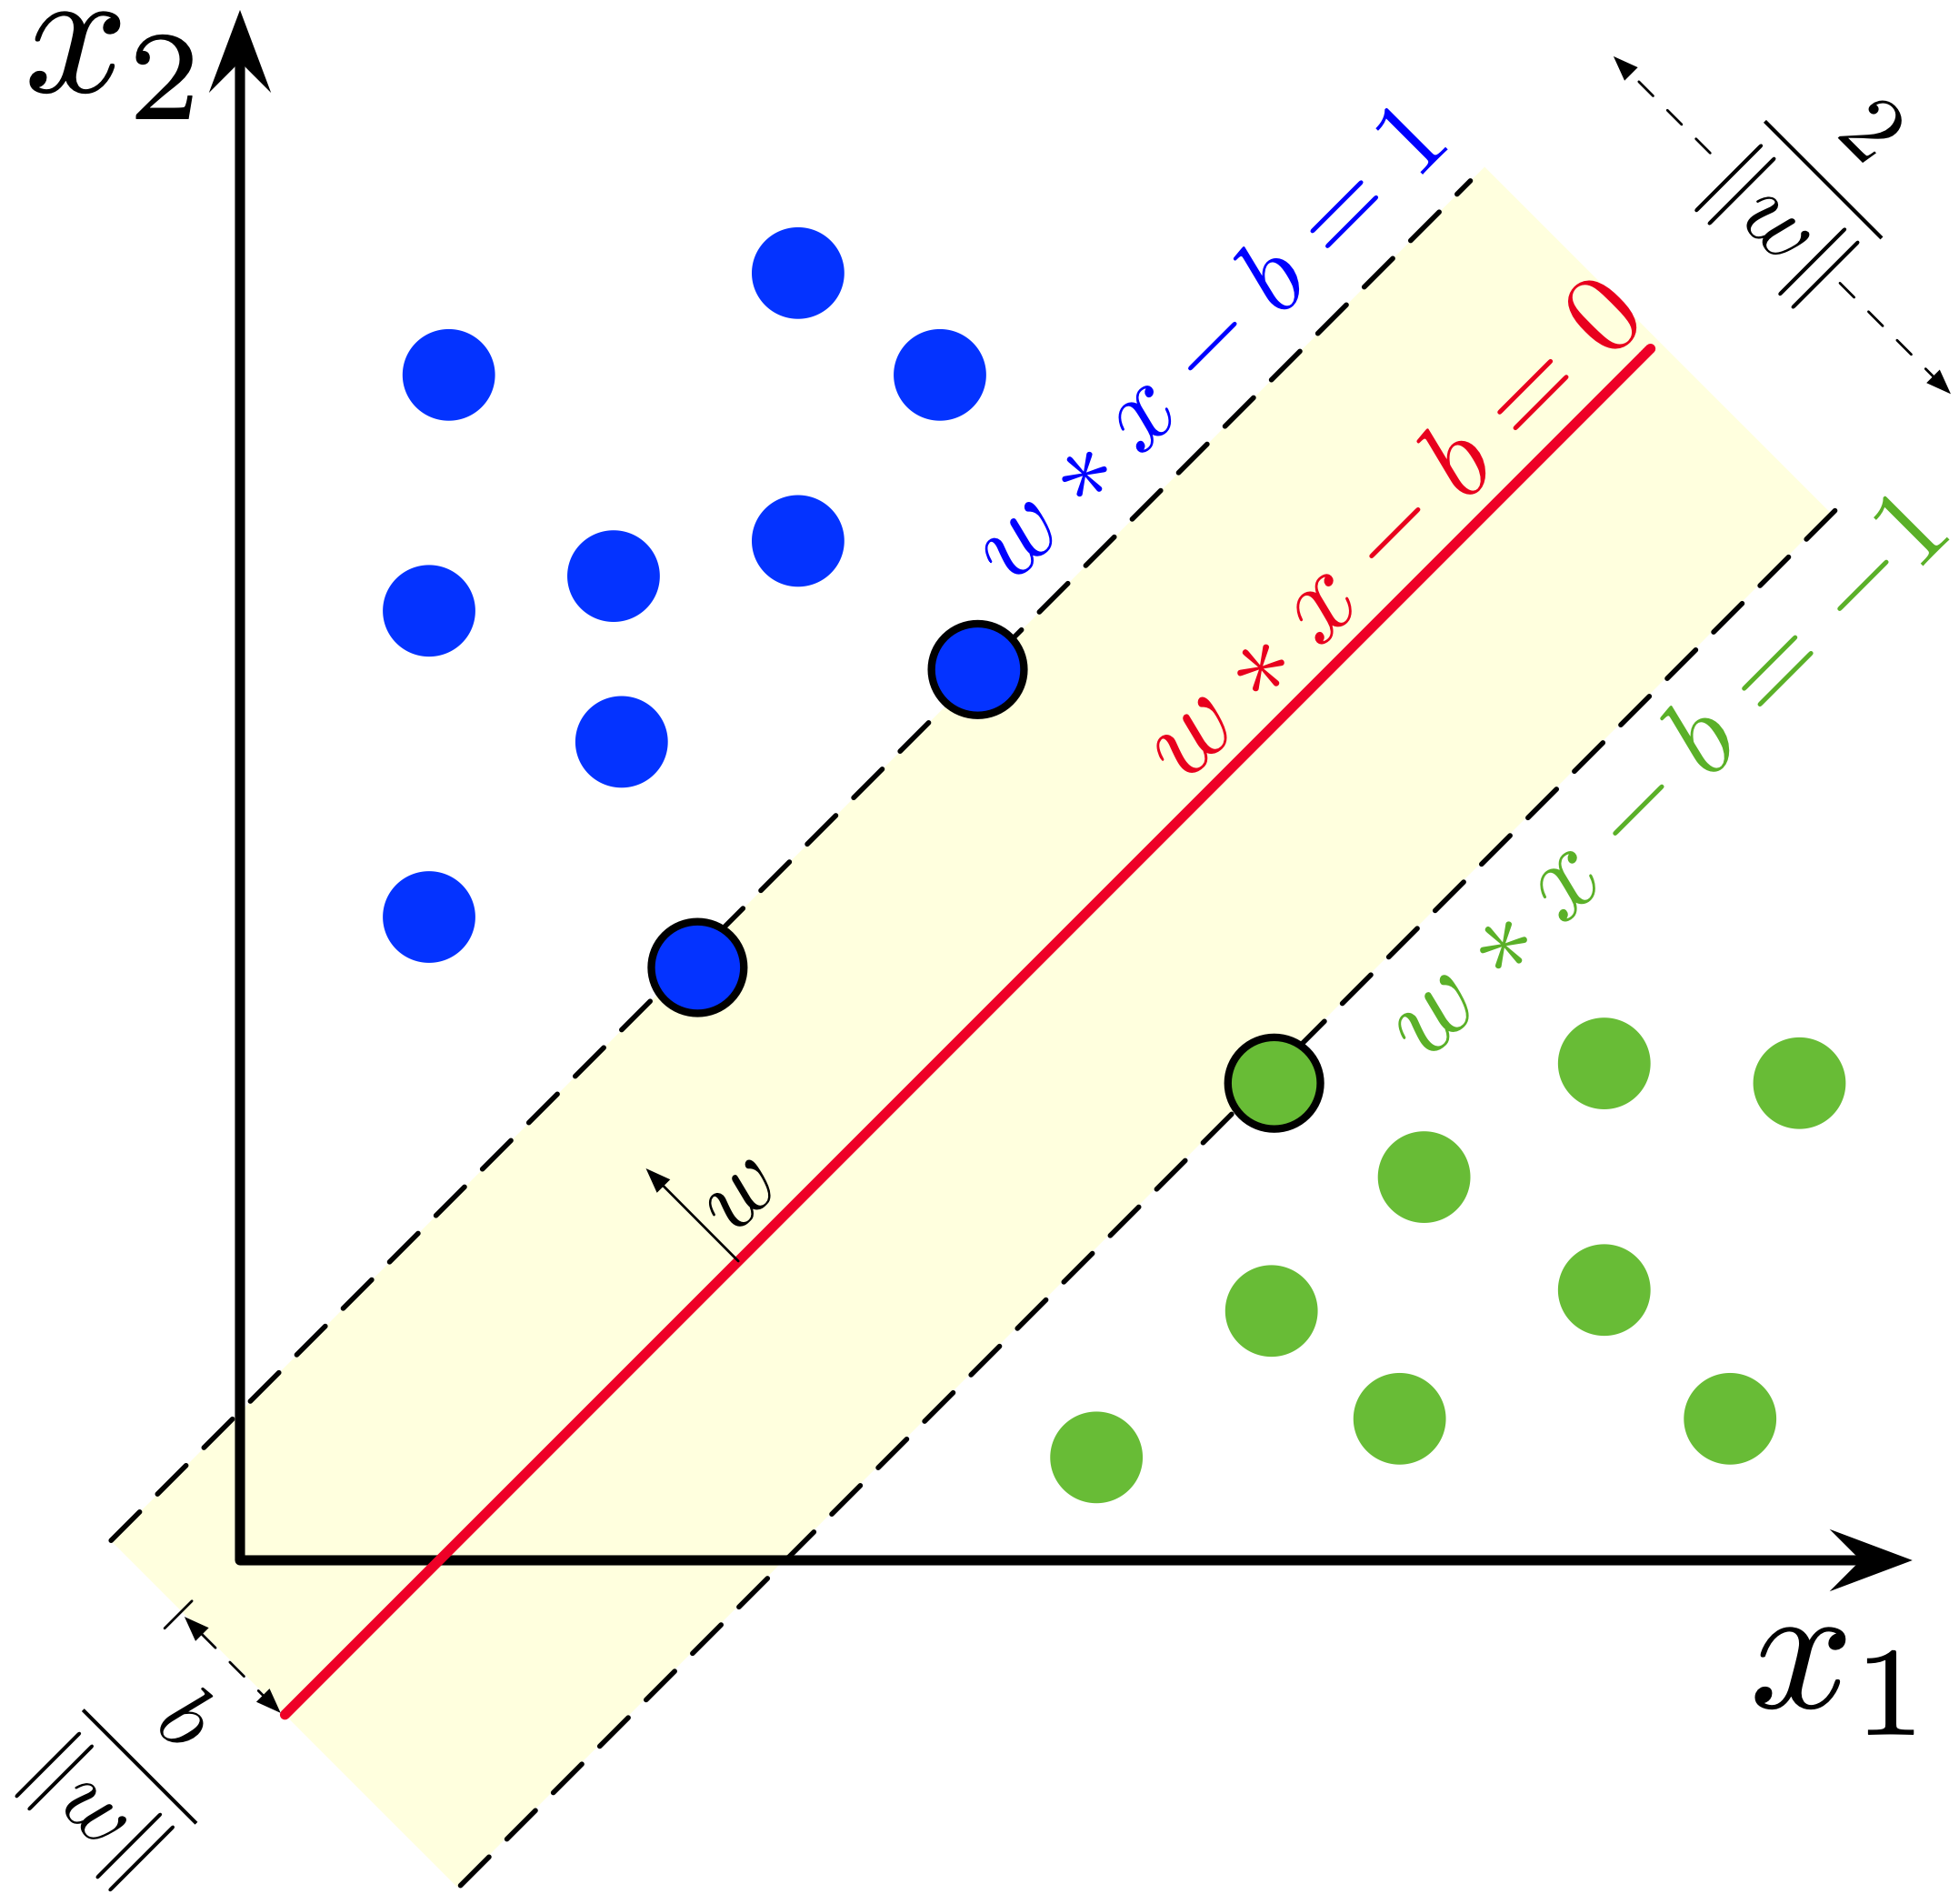
\includegraphics[width=.4\linewidth]{fig/SVM_margin_binary.png}
	\vspace*{2mm}
	\captionfootnotemark{A Hyper-plane and margins of an SVM for a binary classification problem.}
	\label{fig:simple_svm}
\end{figure}
\footnotetext{Retrieved from: \hyperrefurl{https://en.wikipedia.org/wiki/Support-vector_machine} on April 11, 2021.}

A linear SVM hyper-plane is defined as:

\be
\label{eq:linear_hyperplane}
\textbf{w}^{T}\textbf{x} - b = 0,
\ee

where $\textbf{x}$ is a p-dimensional real vector, $\textbf{w}$ is a weight vector normal to the hyper-plane, and b is a real valued bias parameter. Thus the distance between margins can be computed as $\frac{2}{\norm{\textbf{w}}_{2}}$ and we want to maximize it, or inversely we want to minimize $\frac{\norm{\textbf{w}}_{2}}{2}$.

%\subsubsection*{\textit{Loss Functions}}

First, let us name the hyper-plane and margins in Figure~\ref{fig:simple_svm} as:

\begin{itemize}
    \item \textbf{hyper-plane:} 
    \be \label{h0_formula} H_{0} = \textbf{w}^{T}\textbf{x} - b = 0 \:,\ee
    \item \textbf{margin for label +1:}
    \be \label{h+1_formula} H_{+1} = \textbf{w}^{T}\textbf{x} - b = +1 \:,\:\text{and}\ee
    \item \textbf{margin for label -1:}
    \be \label{h-1_formula} H_{-1} = \textbf{w}^{T}\textbf{x} - b = -1 \:.\ee
\end{itemize}

Thus, we have the following condition and result relationships for a p-dimensional sample $\textbf{x}^{i}$ vector with its observed label $y^{i}$ where $y^{i}$ takes either -1 or +1:

\begin{itemize}
    \item if $\textbf{w}^{T}\textbf{x}^{i} - b \geq +1$ and $y^{i} = +1$, then the prediction is correct and the sample belongs to class +1;
    \item else, if $\textbf{w}^{T}\textbf{x}^{i} - b \leq -1$ and $y^{i} = -1$, then the prediction is correct and the sample belongs to class -1;
    \item else, the prediction is incorrect and the sample belongs to opposite of predicted label.
\end{itemize}

When we combine the conditions above, we obtain the following common condition:

\begin{equation}
\label{common_loss} 
1 - (\textbf{w}^{T}\textbf{x}^{i} - b)y^{i} \leq 0\:.
\end{equation}

And finally, the margin perception loss function, called as hinge loss, is written as:

\begin{equation}
\label{hinge_loss} 
loss_{hinge}(\textbf{w}, b) = \sum_{i=1}^{n} \max(0, 1 - (\textbf{w}^{T}\textbf{x}^{i} - b)y^{i}).
\end{equation}

Besides, the squared hinge loss is defined as:

\begin{equation}
\label{squared_hinge_loss} 
loss_{squared\_hinge}(\textbf{w}, b) = \sum_{i=1}^{n} (\max(0, 1 - (\textbf{w}^{T}\textbf{x}^{i} - b)y^{i}))^{2}.
\end{equation}

The constrained optimization problem of SVM is derived as:

\textcolor{red}{yukarida maximization dedin, simdi minimization, bir sonraki denklem de yine max. dilersen hep maksimizasyondan bahsetten, cunku denkleme bakarak minimize mi etmeliyiz, maksimize mi pek anlasilmiyor. \textbf{Ozan:} yukarıdaki hinge ve squared hinge loss'larının tanımları o şekilde olduğu için max'lı yazdım. Primal ve dual problem olarak adlandırılan problemler de equationlarda belirttiğim gibi veriliyorlar hep. Nasıl ve neden bu şekilde yazıldıklarının ayrıntısı için referans vermiştim.}

\be
\label{eq:primal_svm}
\min_{w}\ell(\textbf{w})= \min_{w} \frac{\norm{\textbf{w}}_{2}^{2}}{2} \quad \text{such that} \:\:
(\textbf{w}^{T}\textbf{x}^{i} - b)y^{i} - 1 \geq 0 \:, \quad \forall i \in \{1, ..., n\}
\ee

The equation (\ref{eq:primal_svm}) is called as the primal problem. By using the lagrange function with real valued lagrange multipliers $\alpha_{i}$ greater than or equal to 0, the dual problem to solve is constructed as:

\be
\label{eq:dual_svm}
\max_{\alpha}\Lag(\alpha) = \max_{\alpha} \sum_{i=1}^{n}\alpha_{i} - \frac{1}{2}\sum_{i=1}^{n}\sum_{j=1}^{n}\alpha_{i}\alpha_{j}\:y^{i}y^{i}\:{\textbf{x}^{i}}^{T}\textbf{x}^{j}\quad \text{such that} \:\:\sum_{i=1}^{n}\alpha_{i}y^{i} = 0,
\ee

\textcolor{purple}{where $\Lag$ is the lagrange function, $\textbf{x}_{i}$ and $y_{i}$ are a p-dimensional real valued feature vector and its label, that is -1 or +1, respectively, and $n$ is the number of samples.}

\textcolor{purple}{
An optimization problem can be handle in two perspectives which are the primal problem as the minimization problem and the dual problem as the maximization problem. This kind of optimization problems includes a duality value called as duality gap which is the difference between the lower bound of primal problem and the upper bound of dual problem:}

\be
\text{duality gap} = \text{lower bound}_{\text{primal}} - \text{upper bound}_{\text{dual}}\:.
\ee

\textcolor{purple}{
If $\text{duality gap} = 0$, it is called as strong duality. That is the solution found from either dual or primal problem is the optimal solution of original optimization problem. However, if $\text{duality gap} > 0$, it is called as weak duality and one can try to reduce the duality to zero by using constraints. In that case, the solution of original optimization problem is not the best; but, it can be still used depending on the cost value and tolerance. The illustration of dual and primal problems and duality gap can be viewed in Figure~\ref{fig:duality_gap}.}

\begin{figure}[h]
	\centering
	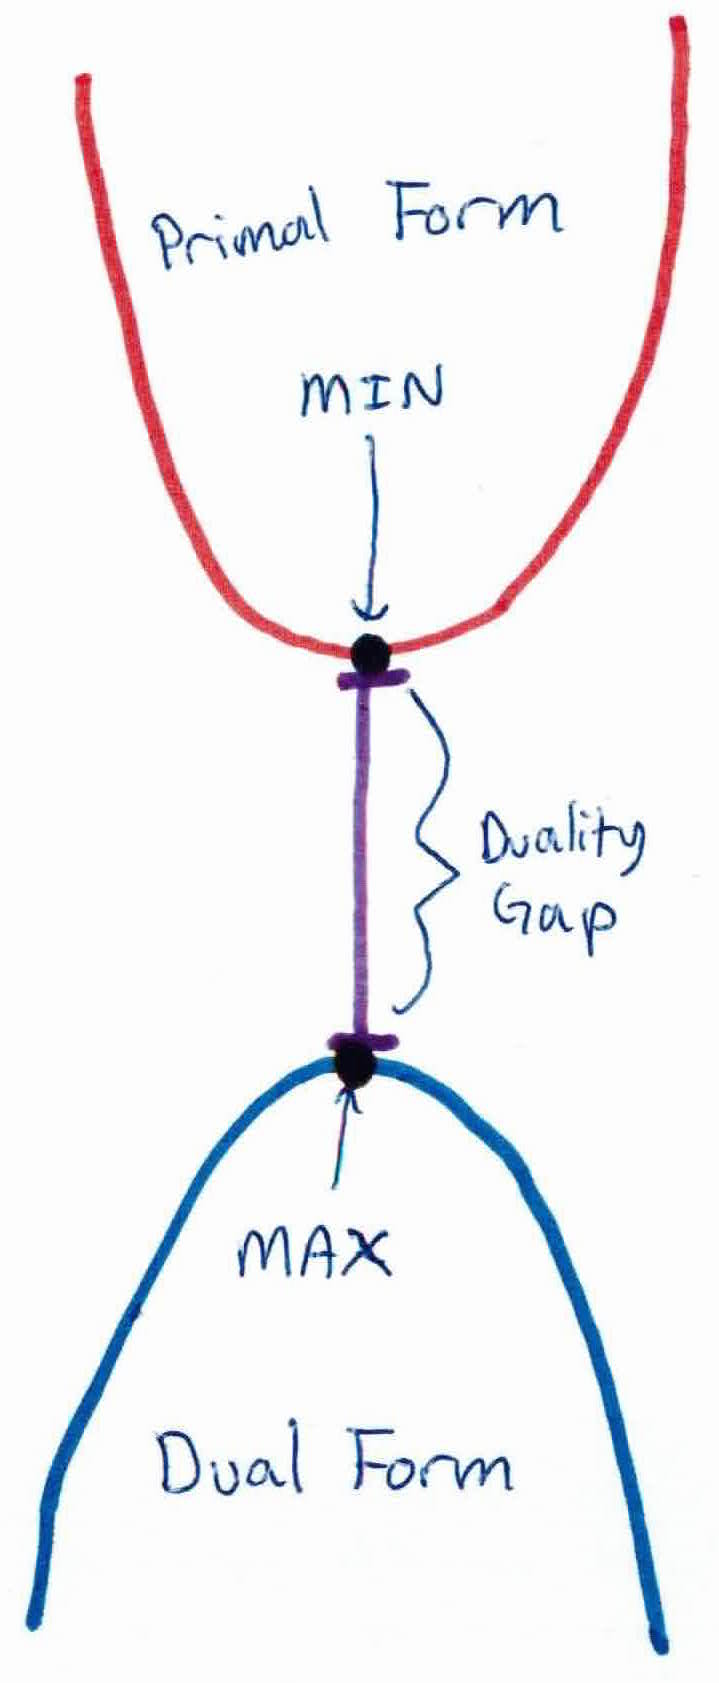
\includegraphics[width=.2\linewidth]{fig/duality_gap.jpg}
	\vspace*{2mm}
	\captionfootnotemark{The dual and primal problems, and the duality gap between their extreme points.}
	\label{fig:duality_gap}
\end{figure}
\footnotetext{Retrieved from: \hyperrefurl{https://kseow.com/svm.html.}}

Further details on constraint optimization of SVM, primal and dual problems and their solutions can be found at  \cite[pg.~13-19]{svm_book}.

\subsubsection*{\textit{Penalty Terms}}
\textcolor{purple}{To decrease the effects of original constraints of SVM problems, and construct more feasible hyper-planes regarding to outlier samples, we use penalty terms adding to original SVM problems. Here $\lambda$ always refers to the regularization parameter, which is a new hyper-parameter to tune, during this subsection.}
\begin{itemize}
    \item \textbf{L2 Regularizer:} According to \cite[pg.~2054-2059]{svm_penalty}, let first recall the primal form of SVM optimization problem in equation (\ref{eq:primal_svm}). We can modify the problem as:
    \textcolor{purple}{
    \be
    \label{eq:l2_svm_primal}
    \min_{\textbf{w}, b} \sum_{i=1}^{n} loss(\textbf{w}, b) + \lambda \frac{\norm{\textbf{w}}_{2}^{2}}{2} ,
    \ee
    }
    
    \textcolor{purple}{where the loss function can be either hinge or squared hinge loss function.}
    
    Then, the corresponding dual problem can be obtained as:
    \be
    \label{eq:l2_svm_dual}
    \max_{\alpha} \sum_{i=1}^{n}\alpha_{i} - \frac{1}{2}\sum_{i=1}^{n}\sum_{j=1}^{n}\alpha_{i}\alpha_{j}\:y^{i}y^{i} \big ( \:{\textbf{x}^{i}}^{T}\textbf{x}^{j} + \lambda \delta_{ij} \big ) \quad \text{such that} \:\:\sum_{i=1}^{n}\alpha_{i}y^{i} = 0\:,
    \ee
    where $\alpha_{i}$ is the lagrange multiplier given in the equation (\ref{eq:dual_svm}) and $\delta_{ij}$ is the Kronecker’s delta function such that it returns $1$ for $i=j$, and $0$ otherwise.
    
    \item \textbf{L1 Regularizer:}
    As stated in \cite[pg.~2054-2059]{svm_penalty}, L1 regularization is only applicable for the linear SVM problem. The L1 penalized SVM optimization problem is given by the following equation where the $loss(\textbf{w}, b)$ is either hinge or squared hinge loss function:
    \be
    \label{eq:l1_svm_primal}
    \min_{\textbf{w}, b} \sum_{i=1}^{n} loss(\textbf{w}, b) + \lambda  \norm{\textbf{w}}_{1}\:.
    \ee
 
    Then, the corresponding dual problem can be obtained as:
    \be
    \label{eq:l1_svm_dual}
    \max_{\alpha} \sum_{i=1}^{n}\alpha_{i} - \frac{1}{2}\sum_{i=1}^{n}\sum_{j=1}^{n}\alpha_{i}\alpha_{j}\:y^{i}y^{i}\:{\textbf{x}^{i}}^{T}\textbf{x}^{j} \quad  \text{such that} \:\:\sum_{i=1}^{n}\alpha_{i}y^{i} = 0 \:\:\text{and}\:\: \alpha_{i} \leq \frac{1}{\lambda}\:,
    \ee
    where $\alpha_{i}$ are lagrange multipliers given in the equation (\ref{eq:dual_svm}), respectively.
    
    
\end{itemize}


\subsubsection*{\textit{Kernel Trick}}

Kernel trick uses a transformation function $\phi(.)$ for mapping samples into a new space so that samples become linearly separable. Then all appearances of samples are replaced with the transformation $\phi(.)$. Now, the kernel function for p-dimensional feature vectors $\textbf{x}_{i}$ and $\textbf{x}_{j}$ is defined as:

\be
\label{eq:kernel_function}
K(\textbf{x}_{i}, \textbf{x}_{j}) = <\phi(\textbf{x}_{i}), \phi(\textbf{x}_{j})> = \phi(\textbf{x}_{i})^{T}\phi(\textbf{x}_{j}).
\ee

This replacement affects the whole structure of SVM optimization problem. The most commonly used kernel functions, which are also used in this thesis, are:

\begin{itemize}
    \item \textbf{Linear function:}
    \be
    \label{eq:lienar_kernel_function}
    K(\textbf{x}_{i}, \textbf{x}_{j}) = \textbf{x}_{i}^{T}\textbf{x}_{j}.
    \ee
    
    \item \textbf{Gaussian radial basis function (RBF):}
    \be
    \label{eq:rbf_kernel_function}
    K(\textbf{x}_{i}, \textbf{x}_{j}) = \exp(-\gamma \norm{\textbf{x}_{i}-\textbf{x}_{j}}_{2}^{2})\:,
    \ee
    for $\gamma >0$. It is common to choose $\gamma =\frac{1}{2\sigma^{2}}$ where $\sigma$ represents the standard deviation of original feature map.
    
    \item \textbf{Sigmoid function:}
    \be
    \label{sigmoid_kernel_function}
    K(\textbf{x}_{i}, \textbf{x}_{j}) = \tanh(\alpha \textbf{x}_{i}^{T}\textbf{x}_{j} + c)\:,
    \ee
    for some $\alpha > 0$ and $c < 0$, and $\tanh(.)$ refers the hyperbolic tangent function.

\end{itemize}

\subsection{Logistic Regression}

%% If the problem contains more than two classes, the model named as Multinomial LR can be used.

Logistic regression (LR) aims to solve binary classification problems.
In the logistic regression model, each sample $\textbf{x} \in \setsymbol{R}^{d}$ has a predicted value $ 0 \leq Pr(\textbf{x}) \leq 1$ referring if the sample belongs to its actual label $y$ or not. If $Pr(\textbf{x})>0.5$, then the prediction is true. By using the logistic sigmoid function, the model is obtained as:

\be
\label{eq:logistic_p}
Pr(\textbf{x}) = \frac{1}{ 1 + e^{-(\textbf{w}^{T}\textbf{x}+b)} }\:,
\ee

where $\textbf{w} \in \setsymbol{R}^{d}$ is the weight parameter tuning the scaling, and $b \in \setsymbol{R}$ is the bias term tuning the shifting in logistic sigmoid function. In the Figure~\ref{logistic_function}, the behaviours of sigmoid function for different $\textbf{w}$ values are given. \textcolor{purple}{Note that, in this figure, the dimensions of samples and weights are one, i.e. $d = 1$.}

\begin{figure}[h]
	\centering
	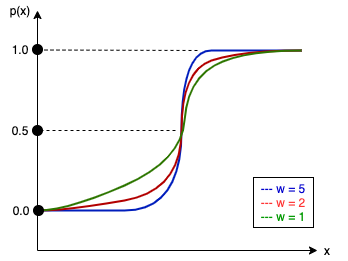
\includegraphics[width=.6\linewidth]{fig/logistic_function.png}
	\vspace*{2mm}
	\caption{Logistic sigmoid function with different scaling w values. }
	\label{logistic_function}
\end{figure}

The sharpness of logistic curve increases with higher $\textbf{w}$ values, and vice versa.

Simply, the hypothesis function can be obtained from sigmoid function as:

\be
\label{eq:logistic_hyptothesis}
\ln \Big (\frac{Pr(\textbf{x})}{1 - Pr(\textbf{x})} \Big ) = \textbf{w}^{T}\textbf{x}+b\:.
\ee

Here, the ratio $\frac{Pr(\textbf{x})}{1 - Pr(\textbf{x})}$ is called as odds, and $\log \Big (\frac{Pr(\textbf{x})}{1 - Pr(\textbf{x})} \Big )$ is the logit function.

For simplicity, let's define $z = \textbf{w}^{T}\textbf{x}+b$. Then, we have the following constraints:

\begin{itemize}
    \item if $y = 1$, we want $Pr(z) \approx 1$, i.e $z >> 0$, and
    \item if $y = 0$, we want $Pr(z) \approx 0$, i.e $z << 0$.
\end{itemize}

\textcolor{red}{>> bu ne demek? \textbf{Ozan:} "çok çok büyüktür"}

Now, we can construct the natural logarithm of the loss function for a sample pair $(\textbf{x}^{i}, y^{i})$ for $i \in \{1, ..., n\}$ as follows:

\begin{equation}
\label{log_loss_onesample} 
loss^{i}(\textbf{w}, b) = -y\ln(Pr(z^{i}))  + (1-y)\ln(1-Pr(z^{i})).
\end{equation}

\textcolor{red}{lossun icine bias niye girdi?yukarıda max l(w) yapmisttin svm de. \textbf{Ozan:} svm'de de hep loss(w,b) olarak yazdım. sadece primal problemde sadece w bulunuyor, orada da primal problemin oluşturulma amacı tek değişkenli loss oluşturmak. Burada da 4.25'in sağ tarafında yer alan z, w ve b'nin functionı olduğu için loss(w,b) olmak zorunda.}


Consequently, the optimization problem is yielded as:

\textcolor{purple}{
\begin{equation}
\label{lr_optimization} 
\min_{\textbf{w}, b} \sum_{i=1}^{n} loss^{i}(\textbf{w}, b).
\end{equation}
}

\subsubsection*{\textit{Penalty Terms}}
\textcolor{purple}{To take the loss function under control by a constraint while constructing the logistic curve separating classes, penalty terms are used.} Here $\lambda$ always refers to the regularization parameter during this subsection.

\textcolor{purple}{
\begin{itemize}
    \item \textbf{L2 Regularizer:}
        \begin{equation}
        \label{lr_l1} 
        \min_{\textbf{w}, b} \sum_{i=1}^{n} loss^{i} + \lambda \norm{w}_{2}^{2}.
        \end{equation}
    \item \textbf{L1 Regularizer:}
        \begin{equation}
        \label{lr_l1} 
        \min_{\textbf{w}, b} \sum_{i=1}^{n} loss^{i} + \lambda \norm{w}_{1}.
        \end{equation}
\end{itemize}
}

\subsubsection*{\textit{Optimizers}}

In this thesis, to solve the optimization problem on LR problem, we use the following solvers presented by scikit-learn package \cite{scikit-learn} in Python programming language:

\begin{itemize}
    \item Newton’s method (newton-cg) \cite{lr_newton_cg}, 
    
    \item Limited-memory Broyden–Fletcher–Goldfarb–Shanno Algorithm \\(lbfgs) \cite{lr_lbfgsb},
    
    \item A library for Large Linear Classification (liblinear) \cite{lr_liblinear},
    
    \item Stochastic average gradient (sag) \cite{lr_sag}, and
    
    \item SAGA \cite{lr_saga}.
\end{itemize}

Different types of optimizers were used for a better approximation to the loss function, and to find the best minimization on this loss function. Table~\ref{tab:lr_solver_table} shows the solvers which are compatible with regularizers.

%% https://stackoverflow.com/questions/38640109/logistic-regression-python-solvers-defintions

\begin{table}[h]
\centering
\caption{Compatibility of logistic regression optimization solvers with regularizers.}
\label{tab:lr_solver_table}
\begin{tabular}{|l|c|c|c|}
\hline
\multicolumn{1}{|c|}{\multirow{2}{*}{\textbf{Solver}    }} & \multicolumn{3}{c|}{\textbf{Regularizer}}                                                                                                                                                                                        \\ \cline{2-4} 
\multicolumn{1}{|c|}{}                        & \multicolumn{1}{l|}{\begin{tabular}[c]{@{}l@{}}No \\ Penalty\end{tabular}} & \multicolumn{1}{l|}{\begin{tabular}[c]{@{}l@{}}L1 \\ Penalty\end{tabular}} & \multicolumn{1}{l|}{\begin{tabular}[c]{@{}l@{}}L2 \\ Penalty\end{tabular}} \\ \hline
newton-cg                                    & \checkmark                                                                          &                                                                            & \checkmark                                                                          \\ \hline
lbfgs                                         & \checkmark                                                                          &                                                                            & \checkmark                                                                          \\ \hline
liblinear                                    &                                                                            & \checkmark                                                                          & \checkmark                                                                          \\ \hline
sag                                         & \checkmark                                                                          &                                                                            & \checkmark                                                                          \\ \hline
saga                                             & \checkmark                                                                          & \checkmark                                                                          & \checkmark                                                                          \\ \hline
\end{tabular}
\end{table}


\subsection{K-Nearest Neighbor}

K-Nearest Neighbor (KNN) is a classification algorithm developed by Fix and Hodges (1951) \cite{knn_pdf}. KNN can be used for regression problems as well; however, at this time, the output for an object is not a class label, but the property value which is the average of the values of its k nearest neighbors. For both usage cases, KNN is a supervised learning algorithm.

\phantomsection
\subsubsection*{\textit{KNN Algorithm}}

Below, the basic algorithm for KNN is explained for n samples $\textbf{x}^{i} \in \setsymbol{R}^{d}$ and their corresponding class labels $c^{i} \in \{-1, +1\}$. Let the target pair is denoted by $(\textbf{x}^{*}, c^{*})$.

\begin{enumerate}
    \item The K nearest neighbors of $\textbf{x}^{*}$ is found with respect to distance between target $\textbf{x}^{*}$ and all other samples. To calculate the distance, different metric functions can be used. The metrics used in this thesis are:
    
    \begin{itemize}
        \item \textbf{Euclidean Distance:}
        \be
        \label{eucledian_distance}
        d(\textbf{x}^{*}, \textbf{x}^{i}) = \sqrt{\sum_{j=1}^{d} ({\textbf{x}^{*}}_{j} - {\textbf{x}^{i}}_{j})^{2}}\:,
        \ee
   
        \item \textbf{Manhattan Distance:}
        \be
        \label{manhattan_distance}
        d(\textbf{x}^{*}, \textbf{x}^{i}) = \sum_{j=1}^{d} |{\textbf{x}^{*}}_{j} - {\textbf{x}^{i}}_{j}|\:, \quad \text{and}
        \ee
        
        \item \textbf{Chebyshev Distance:}
        \be
        \label{chebyshev_distance}
        d(\textbf{x}^{*}, \textbf{x}^{i}) = \max (|{\textbf{x}^{*}}_{1} - {\textbf{x}^{i}}_{1}|, |{\textbf{x}^{*}}_{2} - {\textbf{x}^{i}}_{2}|, \dots, |{\textbf{x}^{*}}_{d} - {\textbf{x}^{i}}_{d}|)\:.
        \ee
    \end{itemize}
    
    \item The class label for $\textbf{x}^{*}$ is estimated by majority voting around K nearest neighbors of target sample found in step 1. Majority voting makes its decision by looking at which class label has the majority in appearance around K nearest neighbors. K is preferred as an odd number. For example, if K is chosen as 3 and these three nearest neighbors have class labels as $\{+1, -1, +1\}$, then the majority voting predicts the target label as +1 since it appears more frequent than label -1. Besides, it can be considered that all of the voters may not have the same effect. In this scenario, one can use weighted majority voting approach which allows the closer neighbor in K nearest neighbors to have the higher effect. That is, the weight of a voter is the multiplicative inverse of its distance to the target sample. For example, assume that the K is chosen as 3 and these three nearest neighbors have class labels as $\{+1, -1, +1\}$ with their distances to the target sample as $\{3, 1, 2\}$, respectively. Then the weights of the neighbors are considered as $\{\frac{1}{3}, 1, \frac{1}{2}\}$ or $\{2, 6, 3\}$ respectively. Here, the label -1 has the majority; thus, the target label is predicted as -1.
\end{enumerate}

\begin{figure}[h]
	\centering
	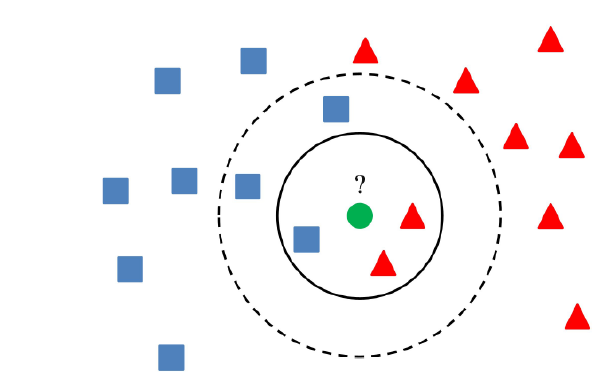
\includegraphics[width=.6\linewidth]{fig/knn_example.png}
	\vspace*{2mm}
	\captionfootnotemark{A KNN example illustration for detecting the class of the green sample.}
	\label{fig:knn_example}
\end{figure}
\footnotetext{Retrieved from: \hyperrefurl{https://ai.plainenglish.io/k-nearest-neighbors-from-scratch-633dfbeac740} on April 17, 2021.}

Figure~\ref{fig:knn_example} illustrates a classification problem for the the sample colored in green. When KNN algorithm with K = 3 is used, the green sample is labeled as red both by majority voting and weighted majority voting. However, when K = 5, use of majority voting or weighted majority voting results in a different label for the green sample. While majority voting labels it as blue,
weighted majority voting labels it as red.

\subsubsection*{\textit{Finding Neighborhood}}

In this thesis, three algorithms presented by scikit-learn
package \cite{scikit-learn} in Python programming language are used to find neighborhoods of samples under KNN algorithm.

%% https://scikit-learn.org/stable/modules/neighbors.html#nearest-neighbor-algorithms
\begin{itemize}
    \item \textbf{Brute Force:} Distances between all pairs of samples are computed. Brute force may be quite efficient for small sized dataset.
    
    \item \textbf{K-dimensional Tree:} When Brute force becomes inefficient as the size of  data set increases, K-dimensional (K-D) tree may be used to reduce the required number of computations. If samples $x_{0}$ and $x_{1}$ are very distant, and samples $x_{1}$ and $x_{2}$ are very close to each other, then we can directly conclude that the samples $x_{0}$ and $x_{2}$ are very distant to each other as well. To create a K-D tree structure, the data space partitioned along the Cartesian axes. Because of the curse of dimensionality, the construction of K-D tree may be inefficient for large dimensions. Further information can be found at \cite{kd_tree}.
    
    \item \textbf{Ball Tree:} Ball tree algorithm was developed to solve the size and dimensionality problems. The data space are partitioned along the spherical axes to construct the tree structure; hence it is more costly than K-D tree. However the structure itself is more effective, especially in high dimensions. Further information can be found at \cite{ball_tree}.
    
\end{itemize}

\subsection{Linear Discriminant Analysis}

The linear discriminant analysis (LDA) is a supervised learning algorithm that is generalized from discriminant analysis developed by Sir Ronald Fisher, who was an statistician, geneticist, and academic, in 1936.

\phantomsection
\subsubsection*{\textit{Derivation}}

A discriminant function $g(\textbf{x})$ from $\setsymbol{R}^{d}$ to $\setsymbol{R}$ is generally a monotonically increasing function defining a boundary between two groups or classes. Here $\textbf{x} \in \setsymbol{R}^{d}$ is a sample with $d$ features and $g_{i}(\textbf{x})$ is the probability of $\textbf{x}$ belonging to class $c_{i}$ over $k$ number of classes as given below:

\be
    \label{eq:prob_x_to_ci}
    g_{i}(\textbf{x}) = Pr(c_{i} | \textbf{x}) = \frac{Pr(\textbf{x}|c_{i}) Pr(c_{i})}{Pr(\textbf{x})}, 
\ee

where $Pr(\textbf{x}|c_{i})$ is the likelihood of observing $\textbf{x}$ given class $c_{i}$, $Pr(c_{i})$ is the prior probability of belonging to class $c_{i}$, $Pr(\textbf{x})$ is the marginal likelihood of observing $\textbf{x}$, \textcolor{purple}{and $i = 1, \dots, k$. Here, we discard the $Pr(\textbf{x})$ since observing $\textbf{x}$ is independent of class.}

We can also take the logarithm of $g(\textbf{x})$ in equation~(\ref{eq:prob_x_to_ci}) since it is monotonically increasing. \textcolor{purple}{Let us re-define the probability function $g_{i}(\textbf{x})$ as:}

\be
\label{eq:log_g}
g_{i}(\textbf{x}) = \ln(Pr(c_{i}|\textbf{x})) = \ln(Pr(\textbf{x}|c_{i})) + \ln(Pr(c_{i}))\:.
\ee

Here, we suppose that the class density $Pr(\textbf{x}|c_{i})$ follows a multivariate normal distribution with mean $\textbf{$\mu$}_{i}$ and variance $\textbf{$\Sigma$}_{i}$ where $\textbf{$\Sigma$}_{i}$ describes class-specific covariance matrix which is generally considered as $\sigma^{2}I$.

\be
\label{eq:normal_distribution}
Pr(\textbf{x}|c_{i}) = \frac{1}{(2\pi)^{d/2}|\textbf{$\Sigma$}_{i}|^{1/2}} \exp \Big[ -\frac{1}{2}(\textbf{x} - \textbf{$\mu$}_{i})^{T}{\textbf{$\Sigma$}_{i}}^{-1}(\textbf{x} - \textbf{$\mu$}_{i}) \Big].
\ee

By inserting equation (\ref{eq:normal_distribution}) into equation (\ref{eq:log_g}), we yield:

\be
\label{eq:prior_linear_disc_func}
g_{i}(\textbf{x}) = -\frac{1}{2}(\textbf{x} - \textbf{$\mu$}_{i})^{T}{\textbf{$\Sigma$}_{i}}^{-1}(\textbf{x} - \textbf{$\mu$}_{i}) -\frac{d}{2}\ln(\frac{\pi}{2}) -\frac{1}{2}\ln|\textbf{$\Sigma$}_{i}| + \ln(Pr(c_{i}))\:.
\ee

Finally, since $\frac{d}{2}\ln(\frac{\pi}{2})$ is constant, we obtain the linear discriminant function for class $i$ as:  \textcolor{red}{genelde i indisini number of samples icin kullandin, ama burada class sayisini indeksliyor. dogru anliyor muyum? \textbf{Ozan:} Evet, yukarıda bunu belirten ifadeler ekledim.}

\textcolor{red}{g(x) logaritması alinmis ifade mi, degil mi dikkatli kullan lutfen, ona gore asagidaki ifadelere tekrar bakiver. \textbf{Ozan:} ben bir çelişki göremedim hocam, siz fark ettiyseniz tartışabiliriz.}
\be
\label{eq:linear_disc_func}
g_{i}(\textbf{x}) = -\frac{1}{2}(\textbf{x} - \textbf{$\mu$}_{i})^{T}{\textbf{$\Sigma$}_{i}}^{-1}(\textbf{x} - \textbf{$\mu$}_{i}) -\frac{1}{2}\ln|\textbf{$\Sigma$}_{i}| + \ln(Pr(c_{i}))\:.
\ee

This linear discriminant function outputs the likelihood of $\textbf{x}$ to be in the class {i}.

There are two presumptive cases on the linear discriminant function which are given below: 

\begin{itemize}
    \item \textbf{$\textbf{$\Sigma$}_{i} = \sigma^{2}I$:} All features have different means, but the same covariance matrix for mathematical convenience. \textcolor{purple}{By replacing $\textbf{$\Sigma$}_{i}$ with $\sigma^{2}I$, we yield the discriminant function as in equation (\ref{linear_disc_func_case1}).}

    \begin{flalign}
        \label{linear_disc_func_case1}
        \nonumber
        g_{i}(\textbf{x}) &= -\frac{1}{2\sigma^{2}}(\textbf{x} - \textbf{$\mu$}_{i})^{T}(\textbf{x} - \textbf{$\mu$}_{i}) -\frac{1}{2}\ln(\sigma^{2d}) + \ln(Pr(c_{i}))\:,\\
        \nonumber
        &= -\frac{1}{2\sigma^{2}}(\textbf{x} - \textbf{$\mu$}_{i})^{T}(\textbf{x} - \textbf{$\mu$}_{i}) + \ln(Pr(c_{i}))\quad \text{since}\:\: \frac{1}{2}\ln(\sigma^{2d})\:\: \text{is constant,}\\
        \nonumber
        &= -\frac{1}{2\sigma^{2}} \big ( \textbf{x}^{T}\textbf{x} - \textbf{x}^{T}\textbf{$\mu$}_{i} - \textbf{$\mu$}_{i}^{T}\textbf{x} - \textbf{$\mu$}_{i}^{T}\textbf{$\mu$}_{i} \big ) + \ln(Pr(c_{i}))\:,\\
        \nonumber
        &= -\frac{1}{2\sigma^{2}} \big ( -2\textbf{x}^{T}\textbf{$\mu$}_{i} - \textbf{$\mu$}_{i}^{T}\textbf{$\mu$}_{i} \big ) + \ln(Pr(c_{i}))\quad \text{since}\:\:\textbf{x}^{T}\textbf{x} \:\: \text{is constant and}\:\: \textbf{x}^{T}\textbf{$\mu$}_{i} = \textbf{$\mu$}_{i}^{T}\textbf{x}\:,\\
        &= \frac{\textbf{$\mu$}_{i}^{T}}{\sigma^{2}}\textbf{x} + \Big (\ln(Pr(c_{i})) -\frac{\textbf{$\mu$}_{i}^{T}\textbf{$\mu$}_{i}}{2\sigma^{2}} \Big ).
    \end{flalign}

It can be seen that, the final discriminant function in equation (\ref{linear_disc_func_case1}) is a linear function. 

    \item \textbf{$\textbf{$\Sigma$}_{i} = \textbf{$\Sigma$}$:} Covariance matrices are all arbitrary, but equal across classes.
    
    \begin{flalign}
        \label{linear_disc_func_case2}
        \nonumber
        g_{i}(\textbf{x}) &= -\frac{1}{2}(\textbf{x} - \textbf{$\mu$}_{i})^{T}\textbf{$\Sigma$}^{-1}(\textbf{x} - \textbf{$\mu$}_{i}) -\frac{1}{2}\ln|\textbf{$\Sigma$}| + \ln(Pr(c_{i}))\:,\\
        \nonumber
        &= -\frac{1}{2}(\textbf{x} - \textbf{$\mu$}_{i})^{T}\textbf{$\Sigma$}^{-1}(\textbf{x} - \textbf{$\mu$}_{i}) + \ln(Pr(c_{i}))\quad \text{since}\:\: \ln|\textbf{$\Sigma$}|\:\: \text{is constant,}\\
        \nonumber
        &= \frac{-1}{2}\big ( \textbf{x}^{T}\textbf{$\Sigma$}^{-1}\textbf{x} - \textbf{$\mu$}_{i}\textbf{$\Sigma$}^{-1}\textbf{x} \textbf{x}^{T}\textbf{$\Sigma$}^{-1}\textbf{$\mu$}_{i} + \textbf{$\mu$}_{i}^{T}\textbf{$\Sigma$}^{-1}\textbf{$\mu$}_{i}\big ) + \ln(Pr(c_{i}))\:.
        \nonumber
    \end{flalign}
    
Since $\textbf{x}^{T}\textbf{$\Sigma$}^{-1}\textbf{x}$ is constant and $\textbf{x}^{T}\textbf{$\Sigma$}^{-1}\textbf{x} = \textbf{$\mu$}_{i}\textbf{$\Sigma$}^{-1}\textbf{x}$, it follows that:   

\begin{flalign}
        g_{i}(\textbf{x}) 
        &= \frac{-1}{2}\big( -2\textbf{x}^{T}\textbf{$\Sigma$}^{-1}\textbf{$\mu$}_{i} + \textbf{$\mu$}_{i}^{T}\textbf{$\Sigma$}^{-1}\textbf{$\mu$}_{i} \big) + \ln(Pr(c_{i}))\quad 
        \nonumber
        \\
        &= \big( \textbf{$\mu$}_{i}^{T}\textbf{$\Sigma$}^{-1} \big) \textbf{x} + \Big(\ln(Pr(c_{i})) -\frac{1}{2}\textbf{$\mu$}_{i}^{T}\textbf{$\Sigma$}^{-1}\textbf{$\mu$}_{i} \Big)\:.
    \end{flalign}

It can be seen that, the final discriminant function in equation (\ref{linear_disc_func_case2}) is a linear function. The illustrations for fixed and varying covariance having data can be found in Figure~\ref{fig:lda_example}.
\end{itemize}
    


\begin{figure}[h]
	\centering
	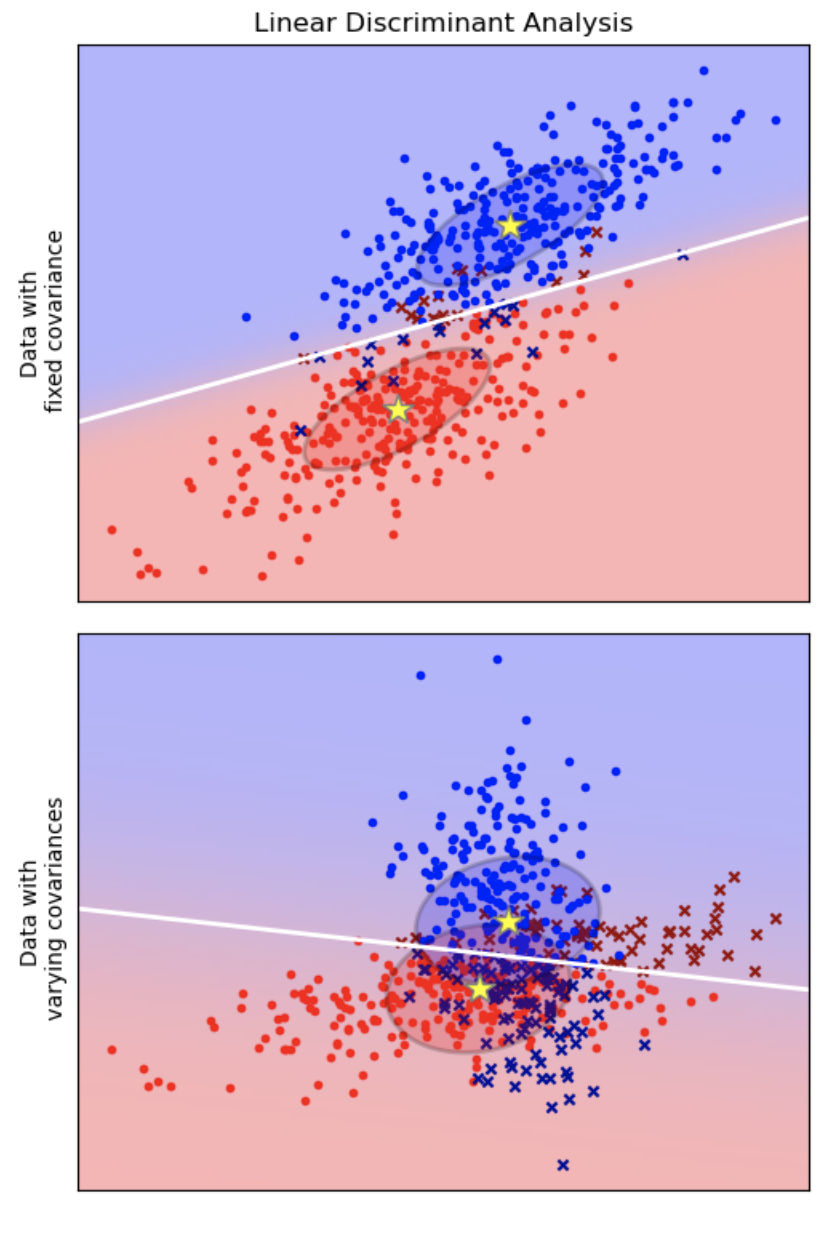
\includegraphics[width=.6\linewidth]{fig/lda.png}
	\captionfootnotemark{LDA process for fixed and varying covariances.}
	\label{fig:lda_example}
\end{figure}
\footnotetext{Retrieved from: \hyperrefurl{https://scikit-learn.org/stable/modules/lda_qda.html} on April 18, 2021.}

\subsubsection*{\textit{Penalty Terms}}
When the number of features is very high, LDA may experience computational difficulties while operating over high-dimensional covariance matrices and then may result in not optimal results. In that case, a simple modification on covariance matrix is made as \cite{regularized_lda}:

\be
\label{cov_regularization}
\widehat{\textbf{$\Sigma$}} = \alpha\textbf{$\Sigma$} + (1-\alpha)I,
\ee

for some real valued $\alpha$ in between the range of $[0, 1]$. We can consider this regularization as what we are used to use in Section~\ref{sec:CH5_regularization}:

\begin{flalign}
    &\widehat{\textbf{$\Sigma$}} = \lambda\textbf{$\Sigma$} + I\quad\text{, or}\\
    &\widehat{\textbf{$\Sigma$}} = \textbf{$\Sigma$} + \lambda I\:,
\end{flalign}

for positive real valued regularization parameter $\lambda$. Consequently, the regularized LDA is formulated as:

\be
\label{eq:regularized_linear_disc_func}
g_{i}(\textbf{x}) = -\frac{1}{2}(\textbf{x} - \textbf{$\mu$}_{i})^{T}{\widehat{\textbf{$\Sigma$}}_{i}}^{-1}(\textbf{x} - \textbf{$\mu$}_{i}) -\frac{1}{2}\ln|\widehat{\textbf{$\Sigma$}}_{i}| + \ln(Pr(c_{i}))\:.
\ee

\subsubsection*{\textit{Solvers}}

In this thesis, to solve the LDA functions, we use the solvers presented by scikit-learn
package \cite{scikit-learn} in Python programming language. Further information about estimators provided by scikit-learn package can be found at \cite{scikit-learn_lda-solvers}.



%% https://scikit-learn.org/stable/modules/lda_qda.html#estimation-algorithms